%! TeX program=latexmk
%! TeX options=-xelatex -synctex=1 -interaction=nonstopmode -file-line-error "%DOC%"
\documentclass[a4paper, nosysfonts]{hpcchina}

\usepackage{graphicx}
\usepackage{amsmath,amsthm}
\usepackage{amssymb,amsfonts}
%以下宏包为测试用途
\usepackage{blindtext}
\usepackage{zhlipsum}
\usepackage{tikz}
\usepackage{metalogo}
%标题
\title{精仿HPC China \XeLaTeX 模板}
%作者
\author{段晓辉\textsuperscript{1,2}}
%单位
\affiliation{
  \textsuperscript{1} 清华大学,北京 100084
  
  \textsuperscript{2} 国家超级计算无锡中心,无锡 214072
}
%邮箱,使用\mailurl{地址}可以生成可点击的链接
\email{\mailurl{sunrise_duan@126.com}}
%中文摘要
\cabstract{
  \zhlipsum[1]
}
%中文关键词
\keyword{
  Latex模板;高性能计算
}
%英文标题
\etitle{DeepFake of HPC China Template in \XeLaTeX}
%英文作者
\eauthor{Xiaohui Duan\textsuperscript{1,2}}
%英文单位
\eaffiliation{
  \textsuperscript{1} (Tsinghua University, Beijing 100084)

  \textsuperscript{2} (National Supercomputing Center in Wuxi, Wuxi 214072)
}
%英文摘要
\eabstract{
  \blindtext[1]
}
%英文关键词
\ekeyword{
  Latex Template; High Performance Computing
}
%基金号
\grants{目前无人捐助此项目}
%DOI号
\doi{missing DOI}
%分类号
\clcls{TP391}
%卷(期):起止页,年
\issue{卷(期):起止页,年}
%收稿日期
\dateaccept{yyyy-mm-dd}
%修回日期
\daterevise{yyyy-mm-dd}
\begin{document}
    \maketitle
    \zhlipsum[10]
    \section{一级标题}
    \zhlipsum[1]
    \subsection{二级标题}
    \zhlipsum[1]
    \subsubsection{三级标题}
    \zhlipsum[10]
    \section{图表}
    \zhlipsum[2]
    \zhlipsum[1]
    %插图还是用figure
    \begin{figure}[!htbp]
      \centering
      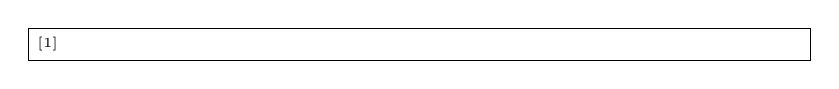
\begin{tikzpicture}
        \node[draw] {\parbox{.8\linewidth}{\tiny\zhlipsum[1]}};
      \end{tikzpicture}
      \caption{一张tikzpicture
        %英文caption用ecaption嵌在caption里面
        \ecaption{A tikzpicture}
      }
    \end{figure}
    \zhlipsum[1]
    %表应该用table也没啥问题
    \begin{table}[!htbp]
      \centering
      \caption{生成奇怪文字所用的库
        \ecaption{Library for generating strange text}
      }
      \begin{tabular}{|c|c|c|}\hline
        语言 & 库 & 命令\\\hline
        中文 & zhlipsum & \verb|\zhlipsum[段落数]|\\\hline
        English & blindtext & \verb|\blindtext[段落数]|\\\hline
      \end{tabular}
    \end{table}
    %表应该用table也没啥问题
    \begin{table}[!htbp]
      \centering
      \caption{ecaption的支持情况
        \ecaption{Supported ecaptions}
      }
      \begin{tabular}{|c|c|c|}\hline
        类型 & 中文 & 英文\\\hline
        figure & 图 x& Fig. x\\\hline
        table & 表 x& Table x\\\hline
        其他 & & 定义方式类似:\\
         &  & \verb|\ecaptionname{figure}{Fig.}|\\\hline
      \end{tabular}
    \end{table}
    \zhlipsum[1-5]
    以一篇古老的分子动力学文章作为参考\cite{jones1924on}
    %参考文献
    \bibliography{ref.bib}
    %作者简介{照片}{文字},可以用includegraphics代替tikzpicture,照片自动缩放
    \authorbio{
      \begin{tikzpicture}\node[minimum width=0.6in, minimum height=0.8in, draw]{照片};\end{tikzpicture}
    }{\textbf{段晓辉} 国家超级计算无锡中心,高级研发工程师,擅长\LaTeX 编程。}


    \authorbio{
      \includegraphics{123.png}
    }{
      This work is licensed under a \href{http://creativecommons.org/licenses/by-nc/4.0/}{Creative Commons Attribution-NonCommercial 4.0 International License}.
    }
\end{document}


